\documentclass{article}
\usepackage{url}  % For URL formatting in references
\usepackage{siunitx} % Provides the \SI{}{} and \si{} command for typesetting SI units
\usepackage{graphicx} % Required for the inclusion of images
\usepackage{tabularx} % Tables
\usepackage[numbers,square]{natbib}
\usepackage{caption}
\captionsetup{width=0.8\textwidth}
\usepackage{amsmath} % Required for some math elements
\usepackage{algorithm2e} % Many options for pseudocode
\usepackage{algorithmic}
\usepackage{listings} % Python code blocks
\usepackage{float} % For better control of figure placement
\usepackage{subcaption}
\usepackage{hyperref}

\setlength\parindent{0pt} % Removes all indentation from paragraphs

\setlength{\parskip}{1em}   % Adjust as desired

\title{Lab 3 Report: Wall-Following on the Racecar} % Title

\author{Team 5 \\\\ Alvin Banh \\ Jialin Chen \\ Jack DeBaugh \\ Haris Imamovic \\ \\ 6.4200: Robotics Science and Systems } % Team # + Names, Class (RSS)

\date{\today} % Date for the report
\renewcommand{\thetable}{\Roman{table}} % Roman numerals for tables, Arabic for figures

\begin{document}

\maketitle

\section{Introduction}
\noindent\textit{Author: Jialin Chen, Editors: Alvin Banh, Jack DeBaugh, Haris Imamovic}

Our goal in this lab was to develop a wall following algorithm and a safety controller for our racecar. Wall following is a method of navigation for autonomous vehicles to traverse terrain without having a predetermined map of its route. This method relies on keeping a desired distance away from the wall at all times. The challenge that comes with wall following is unpredictable geometry and obstacles. However, managing these uncertainties could allow for more self-sufficient autonomous driving behavior.

Using Light Detection and Ranging (LIDAR) sensor data, our team created two different wall-following controllers that can handle various complex environments: Pure Pursuit and Proportional-Integral-Derivative (PID) control. Simultaneously, we created a safety controller that avoids dangerous collisions while not hindering vehicle performance.

Our main challenge when developing a wall-following controller was taking ideal simulation data and replicating ideal behavior in real life. What we ultimately decided for our racecar was a combination of a Pure Pursuit controller for the wall followed by a dynamic safety envelope system.

This report presents our approach to the mathematical principles underlying our wall following algorithms, parameter optimization, and quantitative evaluation. The algorithms used were developed to prevent crashes while maintaining high speeds.

\section{Technical Approach}
\noindent\textit{Authors: Alvin Banh, Jialin Chen, Jack DeBaugh, Haris Imamovic}

\subsection{Technical Problem and System Overview}
The technical problem is creating a vehicle controller to drive a set distance from a wall. This task required detecting the wall's position and generating steering commands. Special cases included doorways, pillars, and corners.

The safety controller must prevent collisions while allowing aggressive driving close to boundaries.

We were given a NVIDIA Jetson controlled mechanical assembly powered by an XTPower 18V battery, driven by a 9v Traxxas motor battery. Although the car build is sturdy and has cushioning in the front to prevent damage when bumping into obstacles, we had to ensure that the robot would not move at velocities at which it could damage itself.  

Our system is implemented using Robot Operating System 2 (ROS2) Humble, leveraging the topic-based communication architecture to separate wall following and safety control into independent nodes.Figure \ref{fig:system_architecture} illustrates the overall system architecture, highlighting the information flow between components~\cite{wall_follower}.

\begin{figure}[H]
\begin{center}
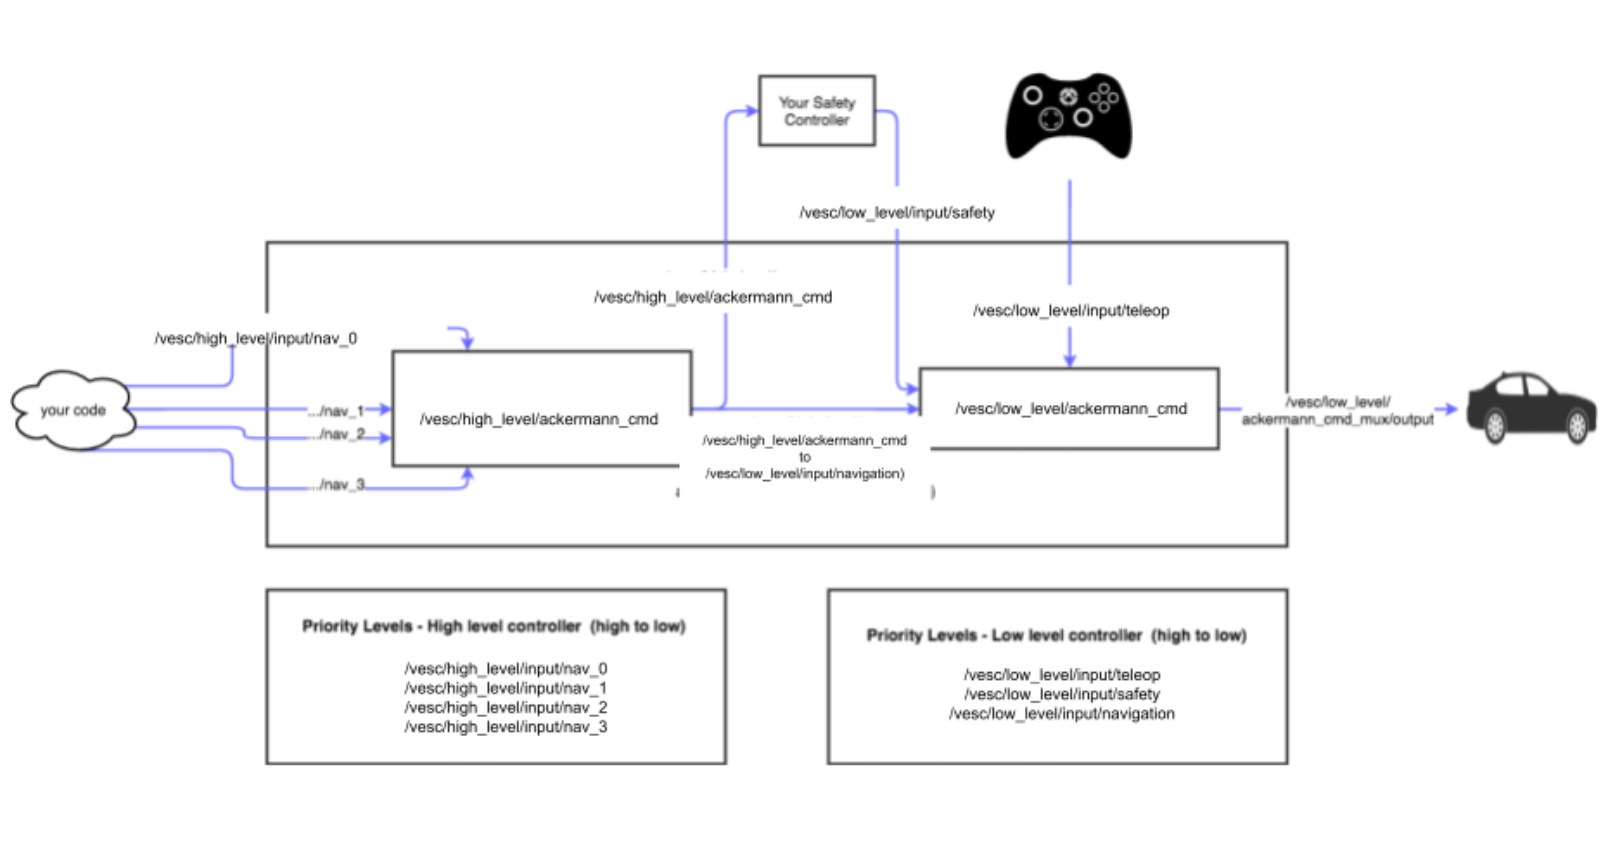
\includegraphics[width=0.85\textwidth]{Muxes.png}
\caption{Command priority architecture of the racecar control system. Higher priority topics override lower priority ones,  with teleop at highest priority.~\cite{wall_follower}.}
\label{fig:system_architecture}
\end{center}
\end{figure}

Our implementation follows a priority-based command structure using the racecar's mux system, where safety commands override navigation commands. Specifically, the wall follower publishes to \texttt{/vesc/high\_level/input/nav\_0} while the safety controller publishes to \texttt{/vesc/low\_level/input/safety}, which has higher priority, overriding wall following in dangerous scenarios.

\subsection{Wall Detection and Line Fitting}
A fundamental challenge in wall following is reliably identifying the wall's position and orientation from LIDAR points while ignoring irrelevant obstacles and features. Our solution extracts a targeted slice of LIDAR data points from the relevant side of the vehicle. Figure \ref{fig:lidar_viz} shows how the slice looks in calculation and how the full LIDAR data points look in simulation.

\begin{figure}[H]
 \centering
    \begin{subfigure}[b]{0.45\textwidth}
        \centering
        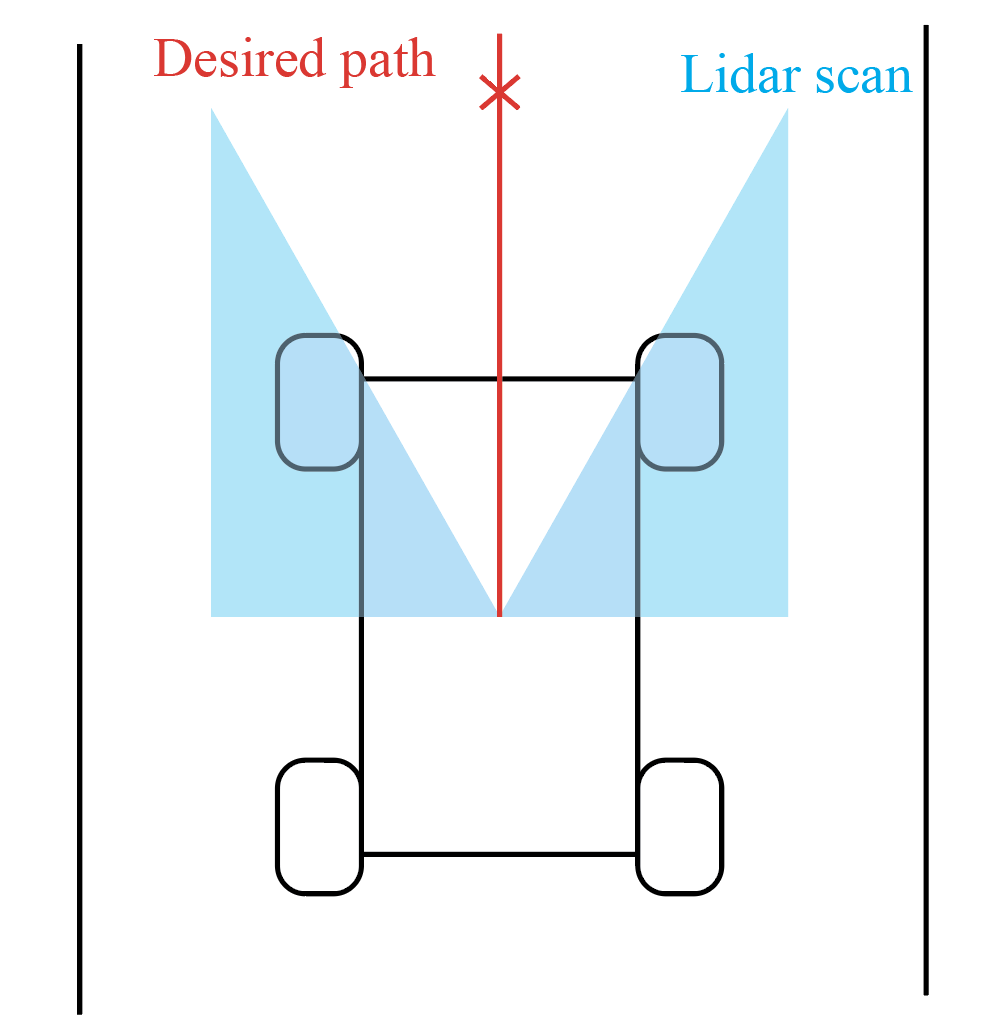
\includegraphics[width=\linewidth]{lidar_scan.png}
        \caption{Sliced lidar scan in blue.}
        \label{fig:lidar_scan}
    \end{subfigure}
    \hfill
    \begin{subfigure}[b]{0.45\textwidth}
        \centering
        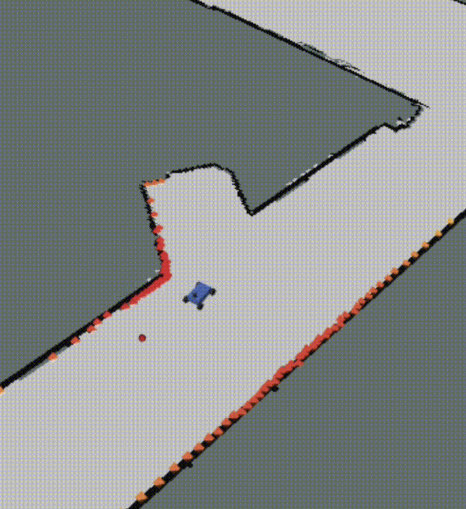
\includegraphics[width=\linewidth]{LookaheadSim.png}
        \caption{Simulated lookahead point.}
        \label{fig:lookahead_sim}
    \end{subfigure}
    \caption{Lidar Scans and Line Fitting Diagrams}
    \label{fig:lidar_viz}
    \hfill
\end{figure}


The wall follower first subscribes to the \texttt{/scan} topic to receive LIDAR data. From this 360° scan, we extract a specific angular slice centered at 70° (for the left side) or -70° (for the right side) with a configurable width. We removed invalid readings (infinite or zero values) and converted to coordinate data in the robot's reference frame.

Using linear regression provides a continuous wall model despite sensor noise and gaps:

\begin{equation}
m = \frac{\sum[(x_i - \bar{x})(y_i - \bar{y})]}{\sum[(x_i - \bar{x})^2]}
\end{equation}

\begin{equation}
c = \bar{y} - m\bar{x}
\end{equation}

Where $\bar{x}$ and $\bar{y}$ are the mean values of the $x$ and $y$ coordinates respectively. This approach handles wall orientation changes smoothly, enabling our system to navigate straight sections and gentle curves. We then offset this line by our desired following distance, creating a target path:

\begin{equation}
c_{offset} = c + d_{offset}\sqrt{1 + m^2}
\end{equation}

\begin{equation}
y_{path} = mx + c_{offset}
\end{equation}

Where $d_{offset}$ is the desired distance from the wall. Due to the robot's coordinate system, for walls on the right, we use a positive offset; for walls on the left, a negative offset. Figure \ref{fig:rviz_line} shows the line of best fit for a right wall. The racecar follows this line.

\begin{figure}[H]
\begin{center}
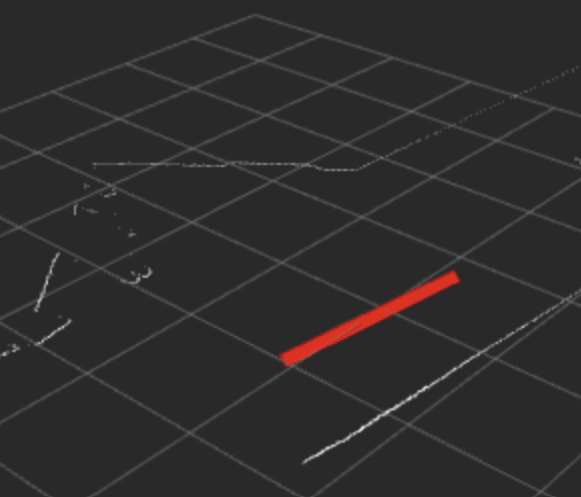
\includegraphics[width=0.5\textwidth]{RViz_SS.png}
\caption{Rviz visualization of the offset line fit is in red. The white points are detected walls.}
\label{fig:rviz_line}
\end{center}
\end{figure}

\subsection{Pure Pursuit Control Strategy}
Converting a target path into smooth, stable steering commands presents a significant challenge, as direct tracking often leads to oscillation shown in PID control. Our approach uses the Pure Pursuit algorithm instead, which selects a point at a fixed distance ahead on the offset path to follow.

We first define a lookahead point at a fixed distance ahead on the offset line:

\begin{equation}
x_L = \text{lookahead $x$ distance}
\end{equation}

\begin{equation}
y_L = mx_L + c_{offset}
\end{equation}

The steering angle is then computed based on the vehicle's position relative to this lookahead point:

\begin{equation}
\alpha = \text{atan2}(y_L, x_L)
\end{equation}

\begin{equation}
L_1 = \sqrt{x_L^2 + y_L^2}=\text{Lookahead distance to point on path}
\end{equation}

\begin{equation}
\text{steering angle} = \text{atan2}(2 \sin(\alpha) d_{wheelbase}, L_1)
\end{equation}

Where $d_{wheelbase}$ is the distance between the front and rear axles of the vehicle. See Figure \ref{fig:pure_pursuit}~\cite{lectures} for the geometry. This approach provides smoother control compared to the PID controller we initially tested, particularly when turning corners.

\begin{figure}[H]
\begin{center}
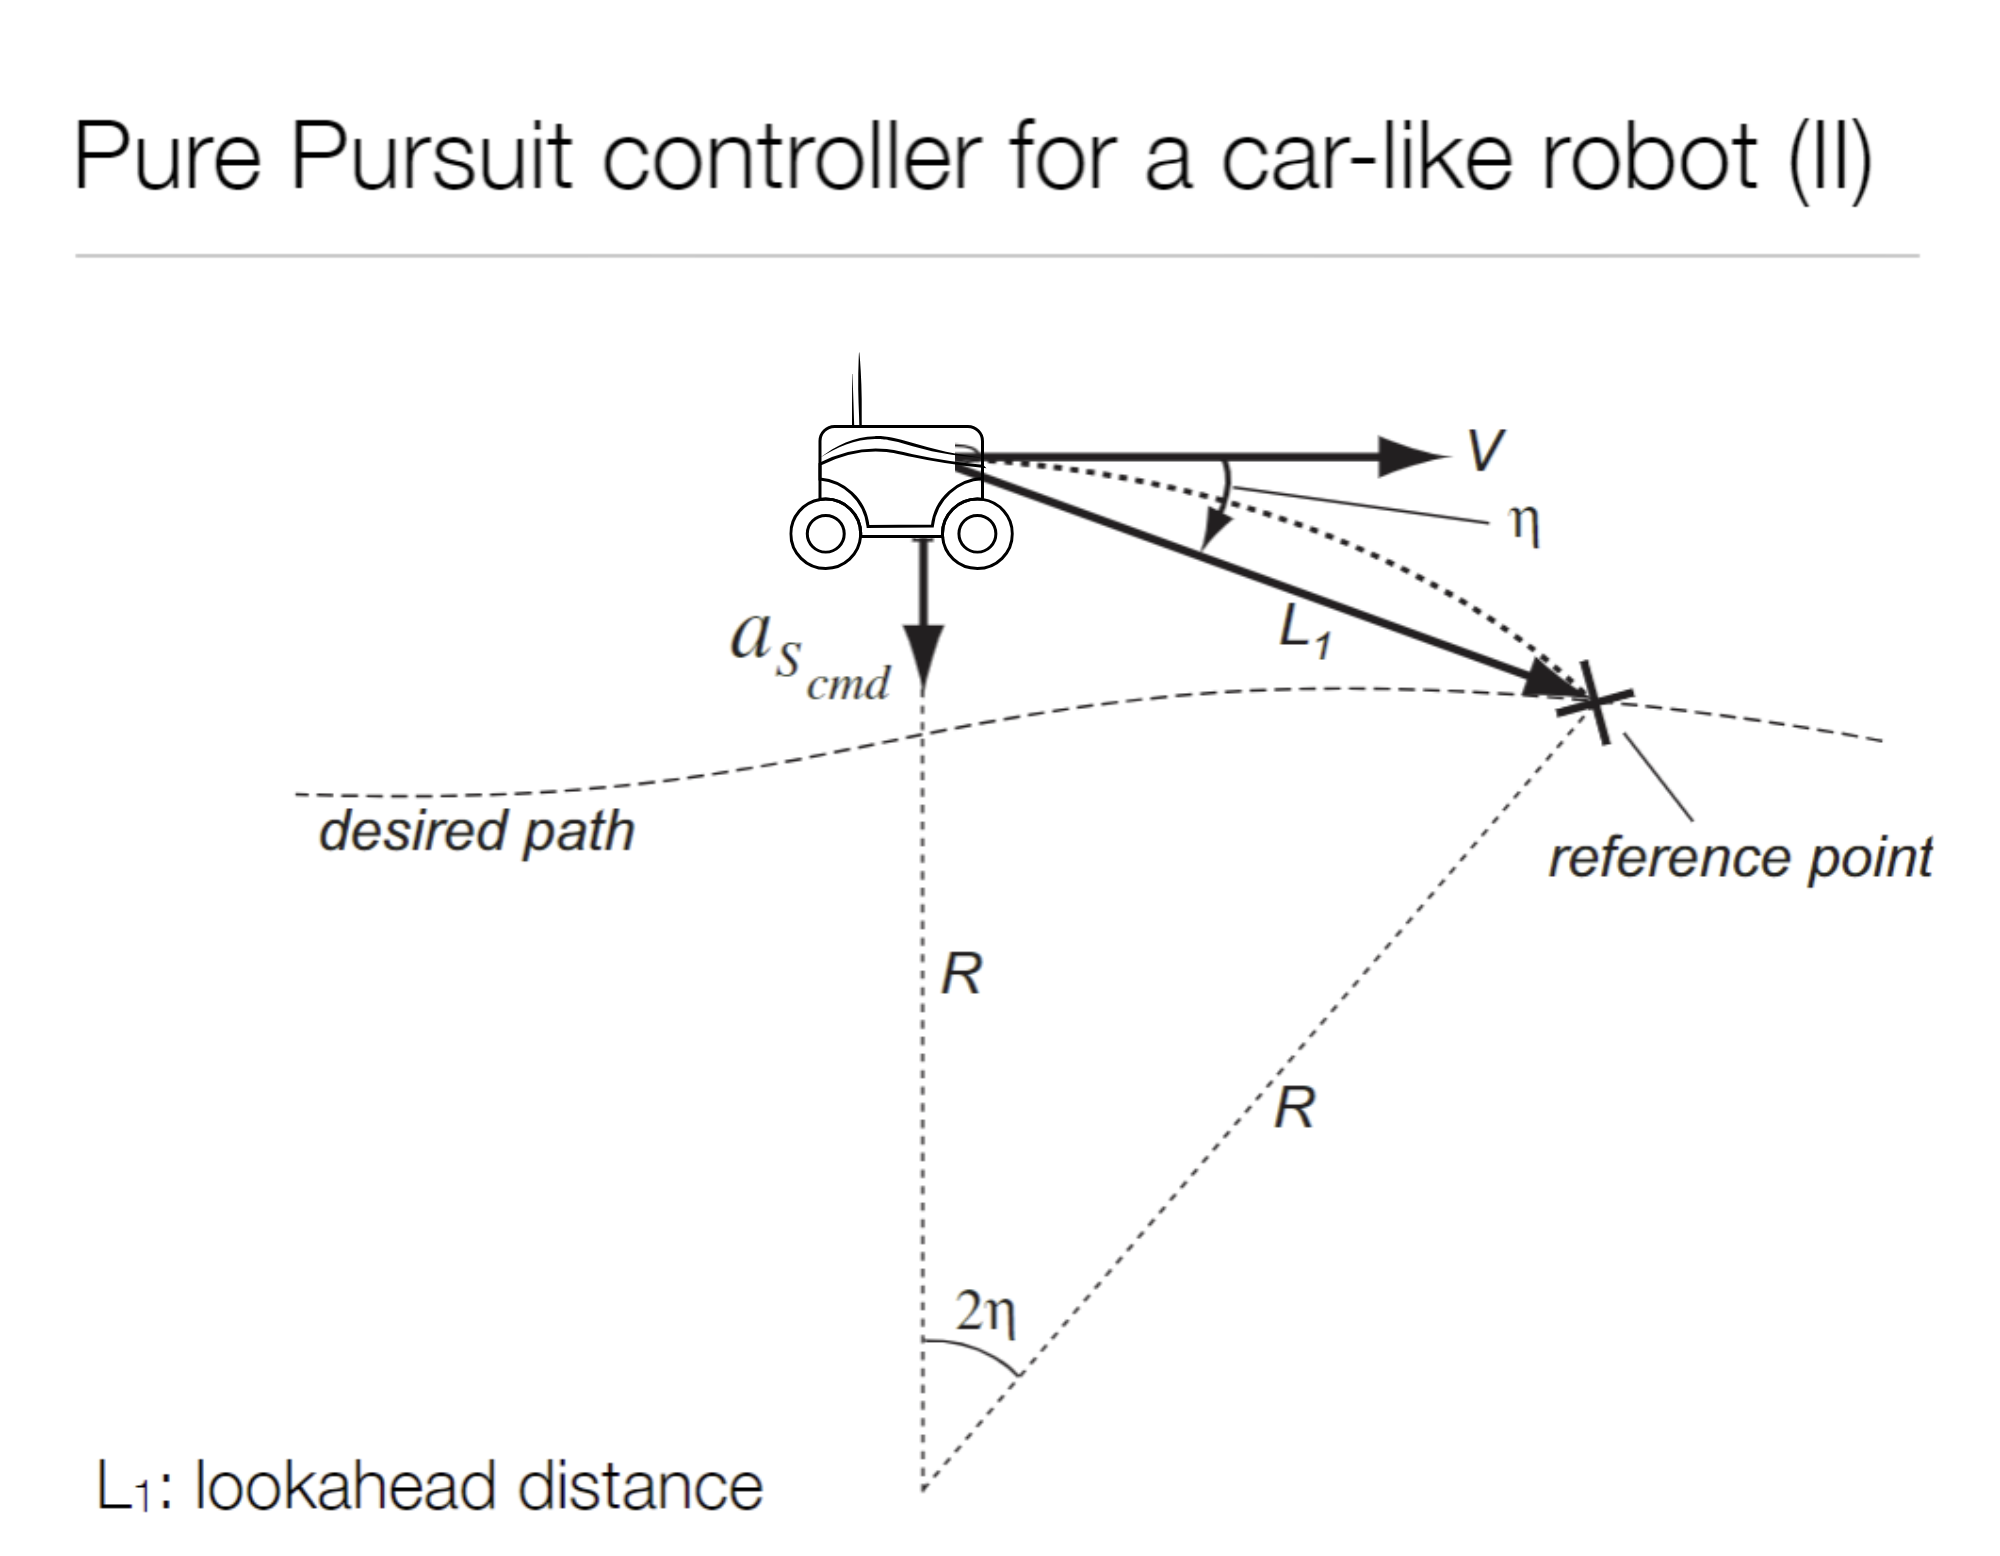
\includegraphics[width=0.75\textwidth]{PurePursuit.png}
\caption{Diagram illustrating the key variables in Pure Pursuit control. The vehicle position, lookahead point ($L_1$), and reference path geometry determine the steering angle ($\delta$) needed to smoothly track the desired path, allowing for predictive rather than reactive control~\cite{lectures}.}
\label{fig:pure_pursuit}
\end{center}
\end{figure}

For internal corners, we implement specialized detection using forward-facing LIDAR data. When the closest point in a narrow forward window is below a threshold distance ($d_{corner}$), we apply a steering offset:

\begin{lstlisting}[language=Python]
def check_forward_obstacle(self, scan_msg):
    half_rad = math.radians(self.FORWARD_HALF_DEG)
    min_front_dist = min(valid)
    if min_front_dist < self.CORNER_DIST:
        return self.CORNER_STEERING_OFFSET * float(self.SIDE)
    else:
        return 0.0
\end{lstlisting}

This approach effectively handles both gradual curves and sharp corners by adjusting the steering behavior based on the environment.

\subsection{Safety Controller Implementation}
A critical challenge in autonomous racing is preventing collisions while still allowing driving aggressively near walls. Our solution projects a dynamic safety envelope that follows the vehicle's anticipated path based on current drive command and LIDAR scans. 

For straight driving (steering angle $\approx 0$), the envelope forms a rectangular projection extending forward by the configurable lookahead distance ($d_{lookahead}$) and a width equal to the vehicle width. For curved paths, we calculate an arcing envelope based on the vehicle's turning radius:

\begin{equation}
R_{turning} = \frac{d_{wheelbase}}{\tan(\text{steering angle})}
\end{equation}

\begin{equation}
\text{Arc sweep} = \frac{d_{lookahead}}{|R_{turning}|}
\end{equation}

\begin{equation}
\text{Envelope boundaries} = |R_{turning}| \pm (0.5w_{car})
\end{equation}

Where $w_{car}$ is the width of the car. Figure \ref{fig:safety_envelope} illustrates how our safety envelope changes shape based on the vehicle's current steering angle.  

\begin{figure}[H]
\begin{center}
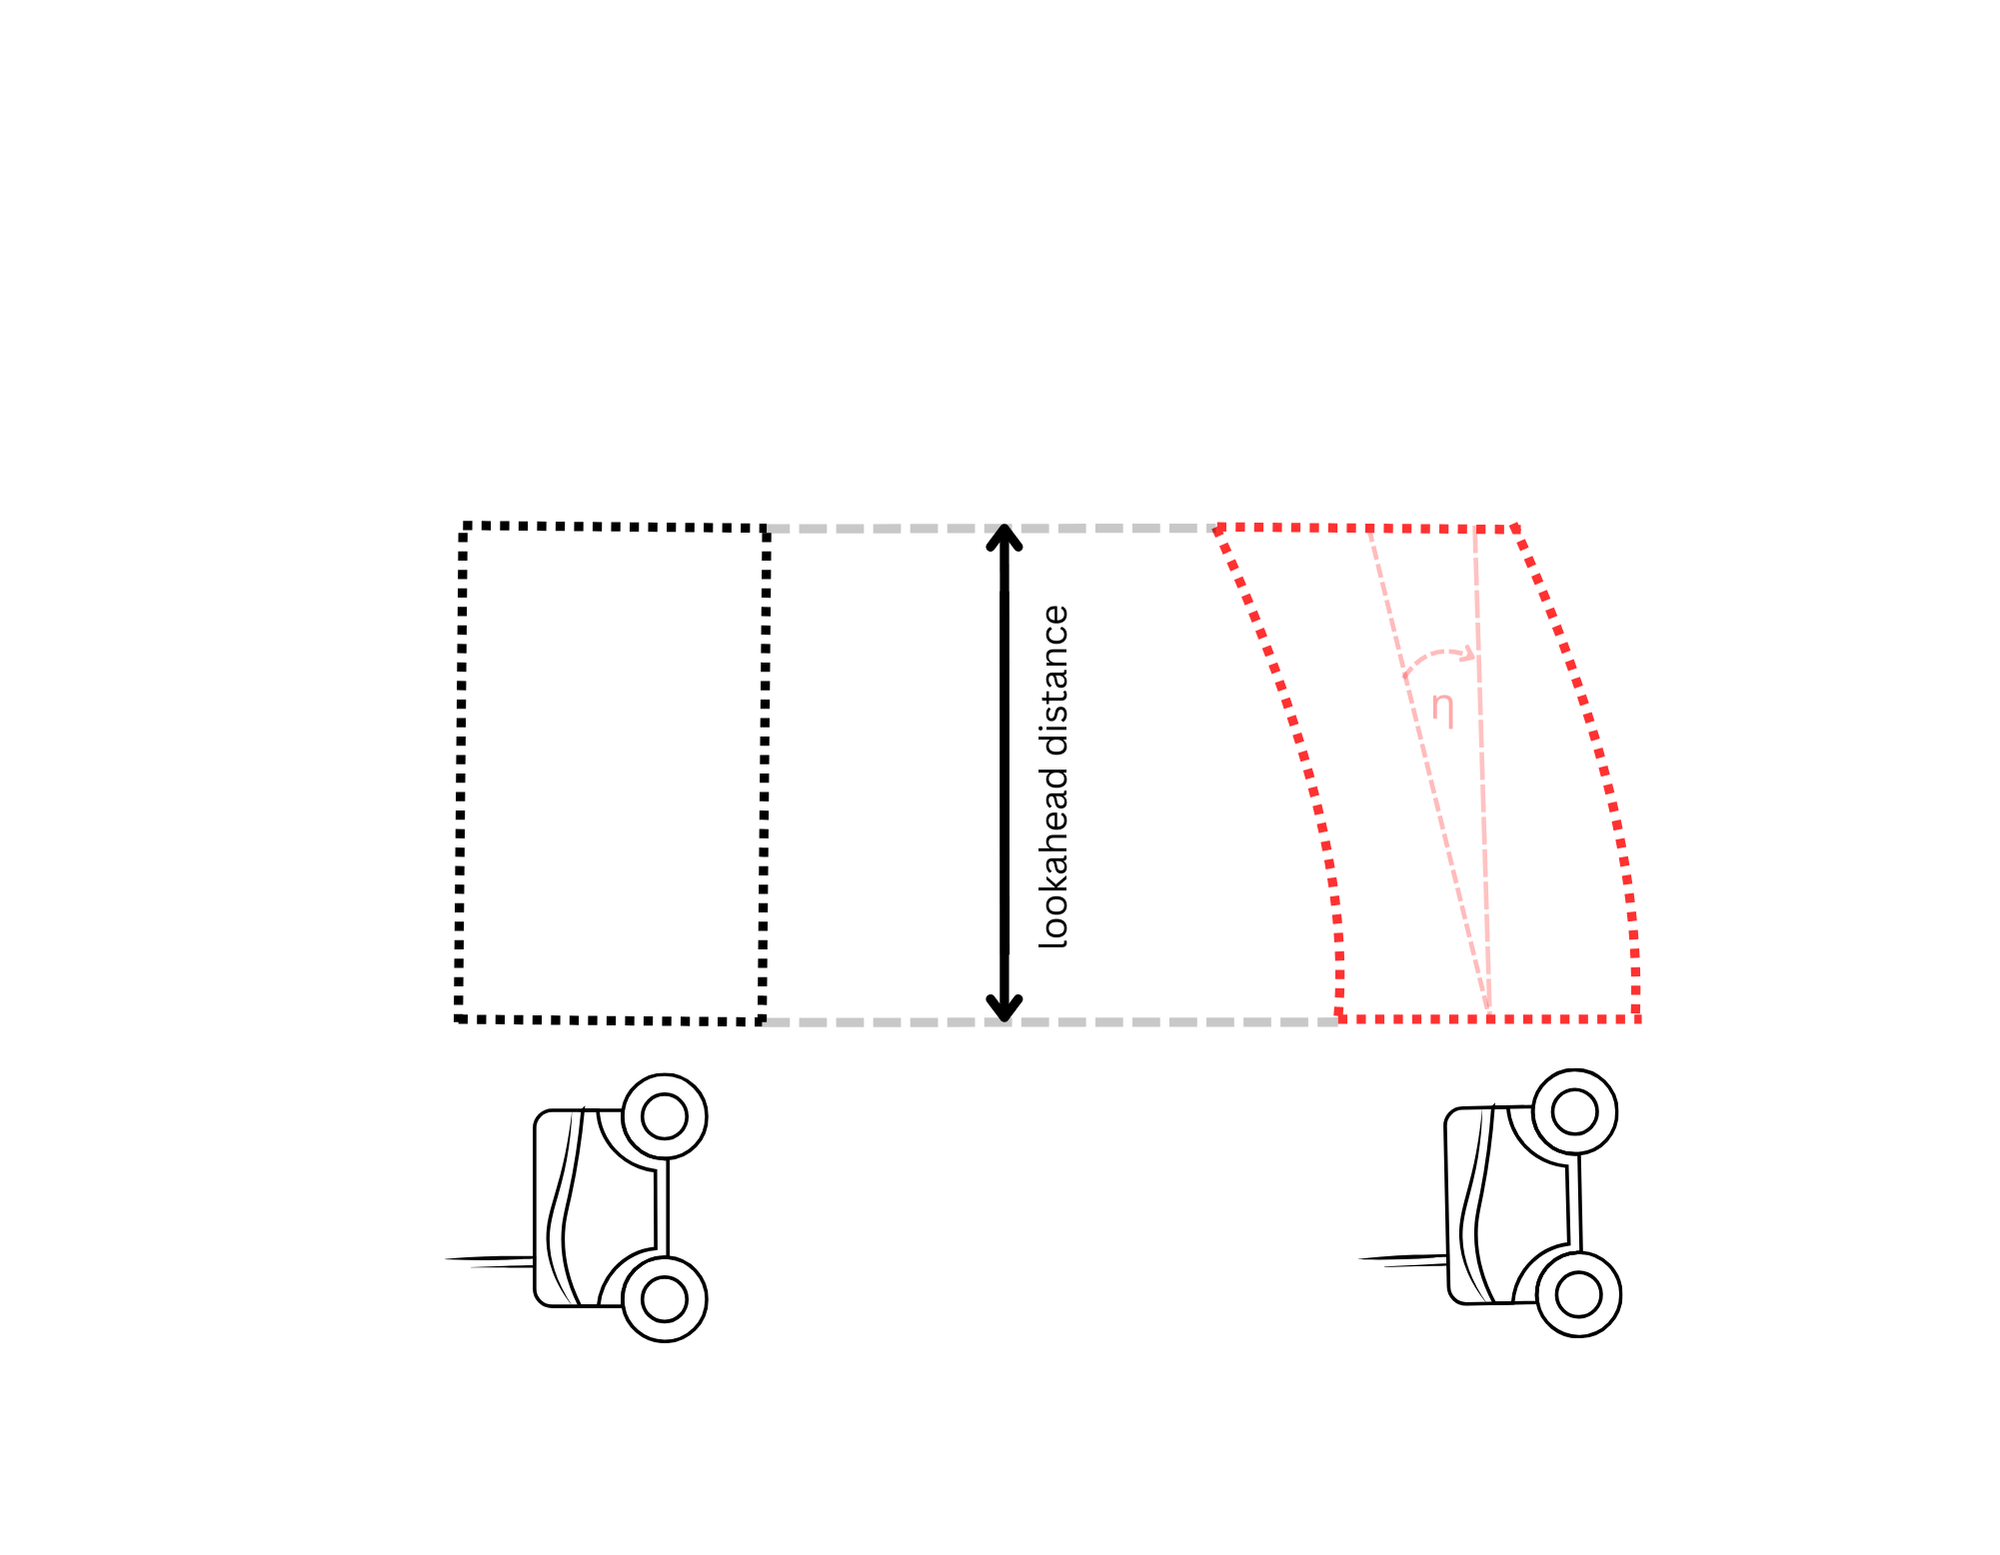
\includegraphics[width=0.85\textwidth]{SafetyController.png}
\caption{Visualization of the dynamic safety envelope concept. Left: A rectangular envelope for straight driving extending ahead with width equal to the vehicle width. Right: An arcing envelope for curved paths based on the vehicle's turning radius. The envelope adapts to the vehicle's current trajectory.}
\label{fig:safety_envelope}
\end{center}
\end{figure}

If more than a threshold number of points are detected inside the envelope, the controller issues an immediate stop command. This approach enables aggressive driving while maintaining safety.

\subsection{Parameter Selection and Tuning}
Several key parameters significantly impact the performance of both systems:

\begin{enumerate}
\item \textbf{Lookahead Distance:} Larger values produce smoother paths but reduce responsiveness to wall variations.
\item \textbf{LIDAR Sweep Width:} Wider angles capture more points but may include irrelevant features; narrower angles may miss important wall sections.
\item \textbf{Safety Envelope Size:} Longer distances provide earlier stopping but may trigger unnecessarily in complex environments.
\item \textbf{Corner Detection Threshold:} Sets the distance at which the system identifies a corner and applies additional steering offset.
\end{enumerate}

We systematically tuned these parameters by balancing quantitative metrics (tracking error, steering variation) with qualitative assessment (smoothness, stability) to determine optimal values.

\section{Experimental Evaluation}
\noindent\textit{Author: Jack DeBaugh, Editors: Alvin Banh, Jialin Chen, Haris Imamovic}

\subsection{Testing Methodology}
We conducted testing on a course in the Stata basement with varying turn angles. Figure \ref{fig:wall_follower_test} shows the live setup and a map of the course. 

\begin{figure}[H]
    \centering
    \begin{subfigure}[b]{0.45\textwidth}
        \centering
        \includegraphics[width=\linewidth]{WallFollowerStartTest.png}
        \caption{Wall follower testing end.}
    \end{subfigure}
    \hfill
    \begin{subfigure}[b]{0.45\textwidth}
        \centering
        \includegraphics[width=\linewidth]{WallFollowerEndTest.png}
        \caption{Wall follower testing end}
    \end{subfigure}
    \hfill
    \begin{subfigure}[b]{0.45\textwidth}
        \centering
        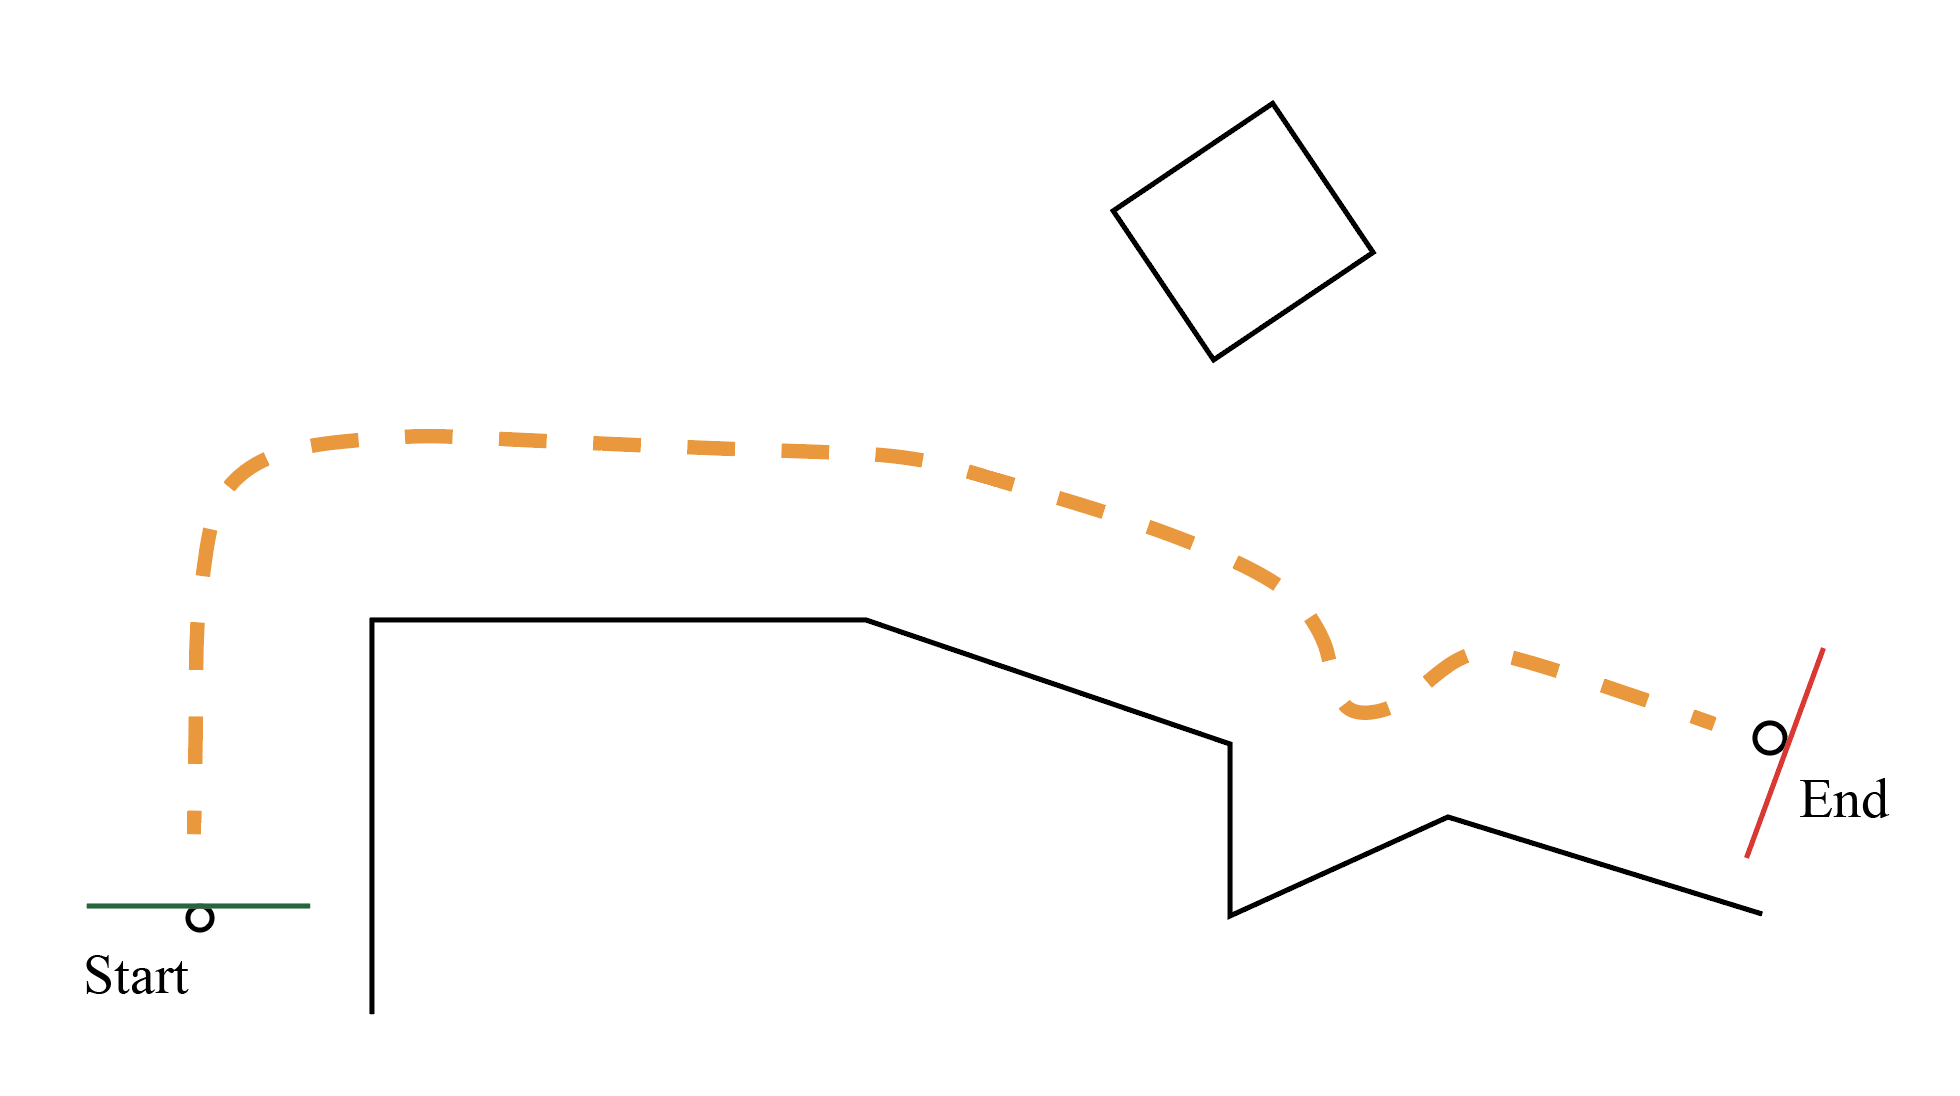
\includegraphics[width=\linewidth]{course_path.png}
        \caption{Bird-eye view of wall follower testing environment.}
    \end{subfigure}
    \hfill
    \caption{Wall Follower Testing Environment}
    \label{fig:wall_follower_test}
\end{figure}

We conducted 12 controlled trials shown in \ref{fig:lidar_sweep}, varying the lookahead distance and sweep width. All tests used the same course at two speeds (0.75 m/s and 1.5 m/s) with a consistent target wall distance (0.5 meters).

\textbf{Performance Metrics}

We evaluated performance using both accuracy and smoothness metrics:
\begin{enumerate}
\item \textbf{Accuracy Metrics:}
   \begin{itemize}
   \item \textbf{Mean Error:} Average absolute deviation from the desired wall distance
   \item \textbf{RMSE:} Root Mean Square Error, emphasizing larger deviations
   \end{itemize}
\item \textbf{Smoothness Metrics:}
   \begin{itemize}
   \item \textbf{Cross-track Error Sign Changes:} Number of oscillations
   \item \textbf{Steering Command Standard Deviation:} Steering variability
   \end{itemize}
\end{enumerate}

We used the LIDAR point $\pm$ 90 degrees from the car to avoid potential errors from line-fitting algorithms.

\subsection{Wall Following Parameter Optimization}

\textbf{LIDAR Sweep Width Optimization}

LIDAR sweep width significantly impacts wall following performance. Figure \ref{fig:lidar_sweep} shows the relationship between sweep width and performance across both testing speeds.

\begin{figure}[H]
\begin{center}
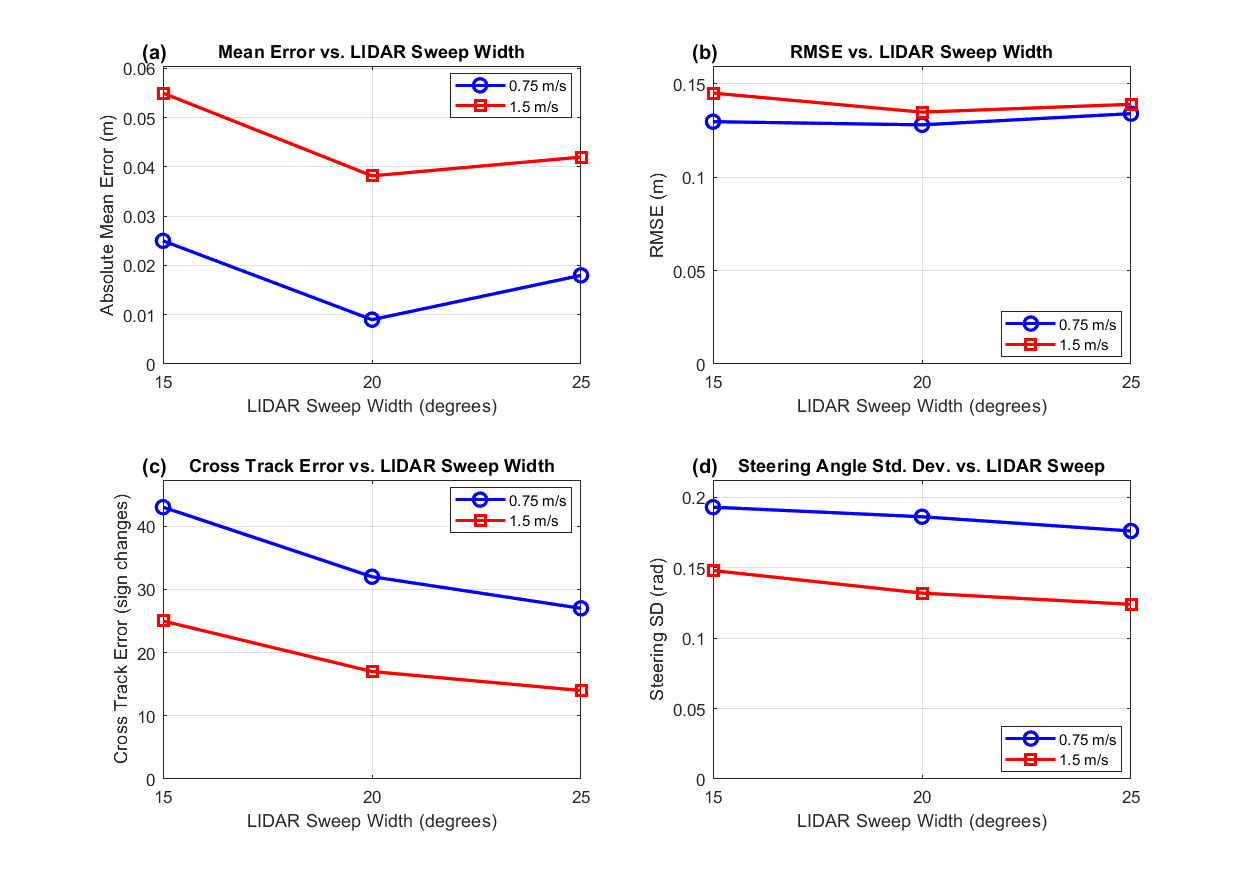
\includegraphics[width=1\textwidth]{FINAL_sweep_plots.png}
\caption{Effect of LIDAR sweep width on wall following performance at 0.75 m/s and 1.5 m/s: While the accuracy metrics, (mean error and RMSE) demonstrate that the 20° setting gathers sufficient data points while avoiding irrelevant environment, smoothness metrics (cross track error and steering angle) show improvement with increased sweep width.}
\label{fig:lidar_sweep}
\end{center}
\end{figure}

Wider sweep angles (25°) produced smoother control but sacrificed accuracy with irrelevant data points. Narrower sweep angles (15°) captured insufficient points for reliable corner detection.

This remained consistent across different vehicle speeds, confirming that 20° represents a robust setting for various racing conditions.

\textbf{Lookahead Distance Optimization}

Figure \ref{fig:lookahead} demonstrates that 1.5 m lookahead distance offers the best balance of accuracy and smoothness. Longer lookahead reduces responsiveness while a shorter lookahead causes more oscillation.

\begin{figure}[H]
\begin{center}
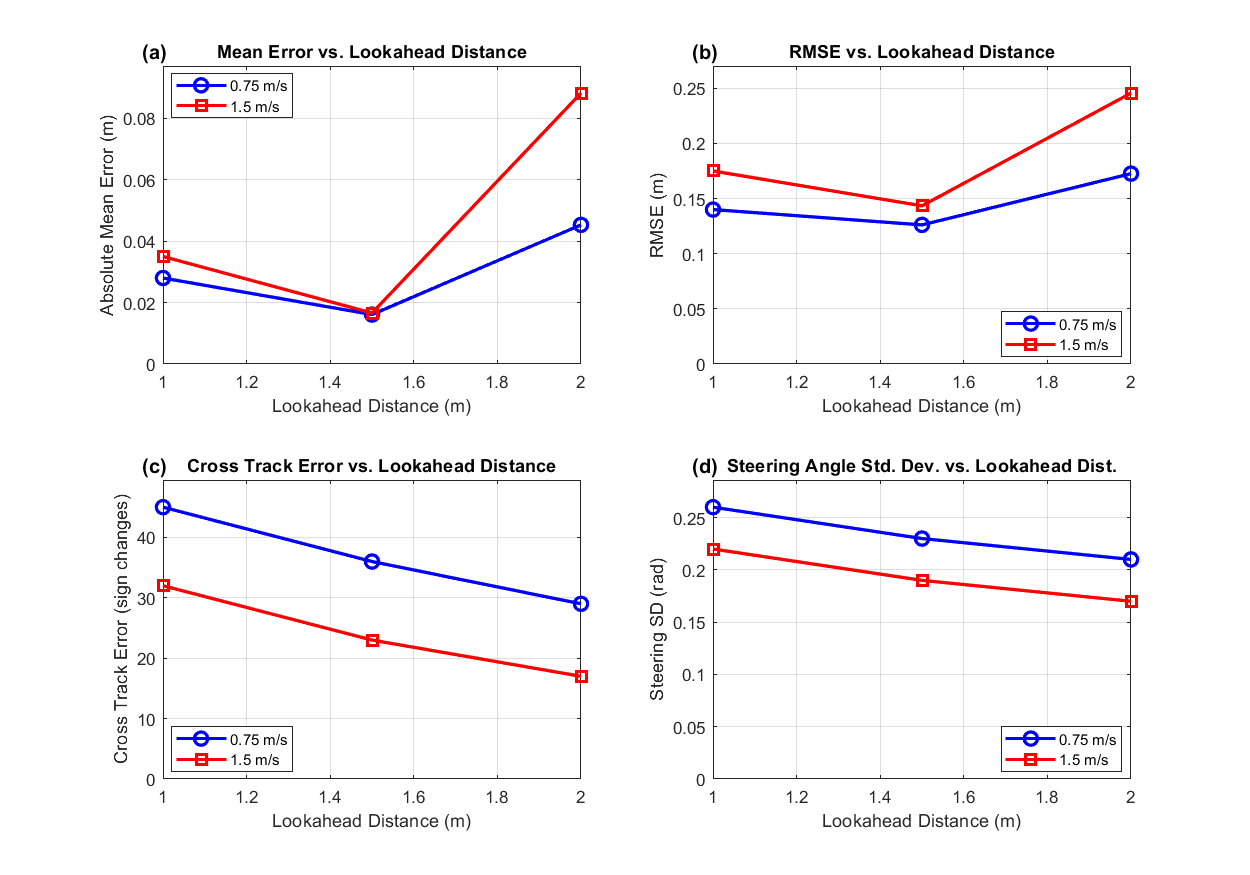
\includegraphics[width=1\textwidth]{FINAL_lookahead_plots.png}
\caption{Effect of lookahead distance on wall following performance metrics at two velocities (0.75 m/s and 1.5 m/s): While accuracy metrics show optimal performance at 1.5 m, smoothness metrics demonstrate improvement as lookahead distance increases, revealing tradeoffs between accuracy and smoothness.}
\label{fig:lookahead}
\end{center}
\end{figure}

This effect was more pronounced at higher speeds, where the 1.5 m setting provided sufficient forward planning while maintaining necessary responsiveness for accurate wall following.

\subsection{Safety Controller Evaluation}

Our testing procedure involved marking a trigger and placement line 33 centimeters apart on the floor, as shown in Figure \ref{fig:safety_controller_test}. When the car crossed the trigger line, an obstacle was placed at the placement line. We measure how far the car traveled before stopping. The videos of these trials can be found \href{https://drive.google.com/drive/folders/1etwTWW4vfrWFXkZLgh6AggkEfVQnLnFo?usp=sharing}{\underline{here}}.




\begin{figure}[H]
\begin{center}
\includegraphics[width=0.6\textwidth]{SafetyControllerTest.png}
\caption{Safety Controller Testing Environment}
\label{fig:safety_controller_test}
\end{center}
\end{figure}


Results showed stopping distances increased with vehicle speed as expected:

\begin{table}[H]
\centering
\caption{Safety Experiment Measurements}
\begin{tabular}{|c|c|c|c|}
\hline
Velocity (m/s) & 0.75 & 1.00 & 1.25 \\
\hline
Stopping Distance (cm) & 13 & 23 & 29 \\
\hline
\end{tabular}
\end{table}

The safety controller achieved 100\% obstacle detection and maintained sufficient margins to prevent collisions. This validates our approach of using a dynamic safety envelope that adapts to the vehicle's expected trajectory based on the turning angle.

\subsection{Qualitative Performance Assessment}
We observed qualitative aspects of our performance through 12 recorded videos ranging from 15 to 30 seconds.

The videos can be found \href{https://youtu.be/PfyAagE1n0A}{here} or at the URL: \url{https://youtu.be/PfyAagE1n0A}.


\section{Conclusion}
\noindent\textit{Author: Alvin Banh, Editor: Jialin Chen, Haris Imamovic}

Our goal was to design a robust wall follower and safety controller, and thus we designed our wall follower utilizing a Pure Pursuit algorithm with a 1.5 m lookahead and a 20° LIDAR sweep on its side. Our experimental results showed we safely followed the wall at the desired distance within 5 centimeters. In addition, our safety controller worked effectively as the stopping distance increases proportional to the velocity. By allowing for more distance to stop, we effectively prevent collisions while not decelerating to a complete stop in the case of a detour path.

Our implementation had challenges with irregular geometries of walls and pillars since our line-fitting was prone to outlier data from the LIDAR scans. In addition, the safety controller could activate in situations that were not necessary, sensing a nonexistent danger. In many of these scenarios, the simulated testing environment in RViz, showed our algorithms working. The difficulty came with deciding what changes to fix behaviors that were not working outside of the simulation.

We plan to implement an improved line-fitting algorithm such as RANSAC for better outlier rejection. In addition, adjusting our calculations to account for our LIDAR's position could be beneficial for inaccurate data handling. Finally, we plan to implement more functionality to our wall-following algorithm with machine learning and vision to predict complex terrain.

\section{Lessons Learned}

\subsection*{Alvin Banh}
A key finding from this lab was to test our systems with robust evaluations without confounding variables. Examples include using better line-fitting algorithms to handle noisy LIDAR data and outliers or charging a battery to full. By using proper tests along the way, we can pinpoint where our algorithms went wrong and course-correct accordingly. It also would help with allowing for more dependable systems that we can abstract for future functionality. A key piece of feedback was to write a testing suite for our software to ensure the reliability of our algorithms and we plan to implement this for future labs. From this experience, I was able to develop skills in collaboration tools such as Git and GitHub to improve our ability to handle software development tasks. I believe I could improve at being more vocal about my schedule and availability as it would streamline our ability to get to a final working product faster.

\subsection*{Jialin Chen}
From late-night testing in the Stata basement, we have depleted our racecar's battery to low numbers a few times and saw unexpected results in drive performance. This includes wall following glitching in with teleop mode and seeing previous code run on the racecar even though new code has been pushed. We also saw really large errors for wall following accuracy when we ran on a low battery to magnitudes that don't make sense with the units we are using, which initially made me doubt the calculations done in the code. However, after fully charging and running the car again, we finally saw numbers that made sense. From this experience, we've learned how to debug as a team and improve in communicating  with each other potential sources of unexpected technical issues. We were able to practice technical communication when talking about how our implementation in code works and potential fixes to cases that failed. In terms of collaboration, figuring out a time that works with everyone and meeting up was very successful and I'm glad that we are consistently doing this.

\subsection*{Jack DeBaugh}
This project revealed a critical disparity between simulation and real-world racecar implementation. Parameters that performed well in simulation required significant adjustment in the physical racecar due to real-world factors like surface friction and sensor noise that weren't accurately modeled. I discovered that early implementation and testing on the physical racecar produced far more reliable results than extended optimization in the simulator. My key takeaway is that developing effective algorithms requires prioritizing real-world testing from the earliest possible stage to ensure that performance meets the requirements. Beyond the technical insights, this project taught me valuable lessons about teamwork and communication. I discovered the critical importance of proper Git usage and strong organizational practices when managing multiple code versions. Going forward I want to do better with organization in that sense so that my teammates can better understand my various code versions. Additionally, I learned that proactively communicating my work schedule and plans significantly improved team coordination, preventing situations where team members worked in isolation without awareness of each other's efforts.

\subsection*{Haris Imamovic}
This initial team assignment provided me with a good insight into working in small teams, as opposed to larger MIT robotics clubs in which I had previously participated. The main difference is the division of work, as each member has a lot more work to complete in a shorter time. I've learned a lot about PID control tuning, and the procedure for determining which coefficients are most optimal, but I've also learned that it is much easier to do it on paper. Testing with an actual robot has a lot more things to consider, like the battery, the physical limitations of the course, etc. Moving forward, we should continue streamlining our division of work, and keep in mind that making a standardized testing procedure will help make the real-life testing conditions easier to navigate. Having only previously taken one course with technical writing, it has been a valuable experience collaborating with the rest of the team. Learning proper technical documentation in a collaborative setting is an essential engineering skill that we've started to spend more time on by applying the feedback we've gotten so far.

\begin{thebibliography}{9}

\bibitem{wall_follower}
MIT RSS Teaching Staff, ``Lab 3: Wall-Following on the Racecar,'' GitHub, 2025. [Online]. Available: \url{https://github.com/mit-rss/wall_follower}. [Accessed: Mar. 12, 2025].

\bibitem{lectures}
MIT RSS Teaching Staff, ``Lecture 5-6: Embedded Control Systems,'' Massachusetts Institute of Technology, 2025. [Unpublished lecture notes].

\end{thebibliography}

\end{document}